\documentclass[12pt,letterpaper]{article}
\usepackage{geometry}
\usepackage[utf8]{inputenc}
\usepackage{natbib}
\usepackage{lscape}
\usepackage{amsmath}
\usepackage{amsfonts}
\usepackage{amssymb}
\usepackage{graphicx}
\usepackage{subfig}
\usepackage{float}
\usepackage{algpseudocode}
\usepackage{fancyhdr}
\usepackage{comment}
\usepackage{hyperref}

\usepackage[english]{babel}
\geometry{verbose,letterpaper,tmargin=3cm,bmargin=3cm,lmargin=2.5cm,rmargin=2.5cm}

% Tables
\usepackage{multirow}
\usepackage[table]{xcolor}

% Avoid to split words at the end of each line
\usepackage[none]{hyphenat}

\usepackage{setspace}

\usepackage{natbib} 
\setcitestyle{numbers,square}

\usepackage{notoccite}


\singlespacing

\begin{document}

% BEGIN TITLE PAGE
\begin{titlepage}

\Large
\sffamily

\begin{center}
  \begin{tabular}{c}
    
\includegraphics[width=0.30\textwidth]{logo-eafit.png}
  \end{tabular}
\end{center}

\vfill
\begin{center}
  \LARGE Title
\end{center}

\vspace*{1cm}
\centerline{\LARGE Alejandro Salazar Arango\footnotemark}  
\footnotetext{Student information (\textcolor{red}{email})}
\vfill

\begin{center}
Advisor(s): \\
Cristhian David Zambrano Mora\footnote{Affiliation, \textcolor{red}{email}}   \\
\end{center}

\vfill

\begin{center}
  \large
    Research practice 3 \\
  Research proposal \\
  Mathematical Engineering\\
  School of Applied Sciences and Engineering\\
  Universidad EAFIT \\
\end{center}

\vfill
\centerline{August 2023}
\vspace*{0.7cm}
\end{titlepage}

% END TITLE PAGE

\section{Introduction}

\begin{comment}

  (\textcolor{red}{4 a 5 párrafos})

Debe incluir:

\begin{itemize}
\item Contexto corto para ubicar al lector.
\item Corta descripción del problema u oportunidad de investigación.
\item Aporte de la investigación.
\item Párrafo que justifique la importancia de la investigación.
\end{itemize}

\end{comment}

Partial differential equations are one of the most powerful tools for the study of physical 
and biological phenomena. They allow us to represent in a simplified way, the dynamics 
between the spatial and temporal variables of any phenomenon and to take this dynamics to a 
mathematical model, whose solution describes in a great way the behavior of the studied 
system\cite{logan2014applied}. This has led partial differential equations to become 
a tool of great use in areas such as fluid dynamics, electromagnetism, optics, magnetism, 
among others\cite{farlow1993partial}; these areas being dominated by PDEs such as Maxwell's 
Equations and Navier-Stokes Equations, the latter being the object of study of the present 
work. \\

However, PDEs, given their complex structure, are usually models whose analytical solutions 
are difficult or impossible to find, being even the solutions already found for some PDEs 
so complex that it is preferred to use other methods to solve the problem\cite{strauss2007partial}. This is why, in 
recent years, the development of multiple numerical methods to solve this type of equations 
has been one of the major topics of study of the scientific community, being this an 
important issue to study, and that although there are already multiple methods developed, 
if these are not applied correctly can lead to solutions far from the real solution of the 
problem and therefore lead to erroneous conclusions about the behavior of the system under 
study.\\

One of the most commontly used numerical method for solving Partial Differential Equations
is the Finite Element Method (FEM), a numerical method consisting on the discretization of
the problem's domain, to later solve a variational formulation of the problem with 
determined test functions, to obtain an algebraic system of equations, which, when solved, 
gives the approximated solution of the problem. However, due to the large amount of degrees 
of freedom it needs in order to correctly solve the PDE, it remains as an extremely 
expensive method both in terms of CPU and memory demand, therefore not being too useful for 
real-time contexts\cite{hesthaven2018non}\cite{PINNQuarteroni}. As a consequence, models 
such as reduced basis models (RBMs) and physically informed neural networks (PINNs) have 
been developed and have become important methods in the study of PDEs.\\

% Parrafo describiendo RBMs y PINNs

This project focuses on the implementation of artificial intelligence models for the solution of 
PDEs, specifically Physical Informed Neural Networks (PINNs) and Neural Network asisted Reduced 
Basis Models (NN-RBM), seeking to obtain a reduced computational cost in a real-time simulation 
context. The Navier-Stokes equations, and in particular, a simulation problem of blood flow through 
the carotid artery, will be used as an object of study, to observe and compare the performance of 
these methods versus the FEM in an on-line simulation process, aiming for a deeper understanding of the advantages and limitations of NN-RBMs, PINNs and FEM in the context of real-time simulations.

\begin{comment}
  Parrafo comentando los principales métodos implementados en CFD (principamente FEM) comentar el alto número de grados de libertad e introducir RBM y PINN utilizando NN.
  
  Parrafo comentando rápidamente el objetivo de la investigación, como se realizará y el aporte esperado.
\end{comment}

\section{Statement of the problem}



\subsection{Statement of the problem}

\begin{comment}
  \textcolor{red}{4 a 5 párrafos})
  En este apartado debemos ampliar la descripción del problema.

  En esta subsección se hace una ampliación del problema descrito en la introducción. Acá hay
  algunas aspectos que se pueden abordar acá.

  \begin{itemize}
 \item En algunos casos, un problema tiene diferentes nombres en la literatura. En estos casos es bueno contarle al lector con qué otros nombre se conoce el problema en diferentes áreas de conocimiento.
 \item Si es una investigación aplicada, es conveniente pensar en que matices o particularidades adquiere el problema al aplicarse en un contexto específico. Puede que lo que no sea un problema en un lugar si lo sea en otro.
 \item ¿A quienes afecta el problema?¿a qué escala opera? (grupos poblacionales, zonas geográficas, período temporal: pasado, actual o futuro).
 \item ¿Qué desencadena o genera el problema?
 \item ¿Qué repercusiones o efectos tiene el problema?
 \item ¿Se han postulado soluciones a este problema pero no lo suficientemente satisfactorias?
\end{itemize}

\end{comment}


For solving fluid dynamics problems, Computational Fluid Dynamics (CFD) mainly uses three methods: The Finite Difference Method, The Finite Volumes Method, and the Finite Element Method. In the finite difference method, the derivatives of the problem are usually replaced by truncated expansions of the Taylor series, this method is straightforward for regular geometries, but when working with irregular geometries it is necessary to perform transformations to the equations before the expansion is carried out\cite{AutoDesk}. In the finite volume method, the discretization is performed by partitioning the spatial domain into a mesh, in which each of its elements will be called a control volume. The idea is to perform the integration of the dominant equations of the problem through each control volume, balancing the fluxes across the boundaries of the individual volumes and getting what is called a balance equation. Then the set of balance equations will be discretized with respect to a set of discrete unknowns to finally get the solution to the problem\cite{volumes}. In a topologically regular mesh, these calculations are done quite easily, but when working with irregular meshes, this calculation will result in an unbearable amount of fluxes and a significant accounting effort to ensure that all fluxes have been calculated correctly\cite{AutoDesk}.\\

Finally, the finite element method is a numerical method highly used in computational fluid dynamics to solve problems whose domain is defined by irregular geometries. The method makes it possible to find the numerical solution to these problems by dividing the initial domain of the same (a continuous element) into a large number of non-intersecting subdomains, called finite elements. Each element will have a set of representative points called nodes, which will make up the complete grid of the problem, on which the calculations will be performed. At last, the formulation of a boundary value problem ends up giving a system of algebraic equations, which are then solved using variational methods in order to approximate a solution, minimizing an associated error function\cite{element}.\\



\subsection{Formalization of the problem}

\begin{comment}
  En esta subsección debén escribir una descripción más formal, muy al grano,
del problema.  Se deben incluir los principales elementos matemáticos que
tiene el problema.  En la siguiente figura hay un ejemplo de formalización del
problema tomado de Duque, J. C., Anselin, L., \& Rey, S. J. (2012). The
max‐p‐regions problem. Journal of Regional Science, 52(3), 397-419.


 \begin{center}
  \begin{tabular}{c}
    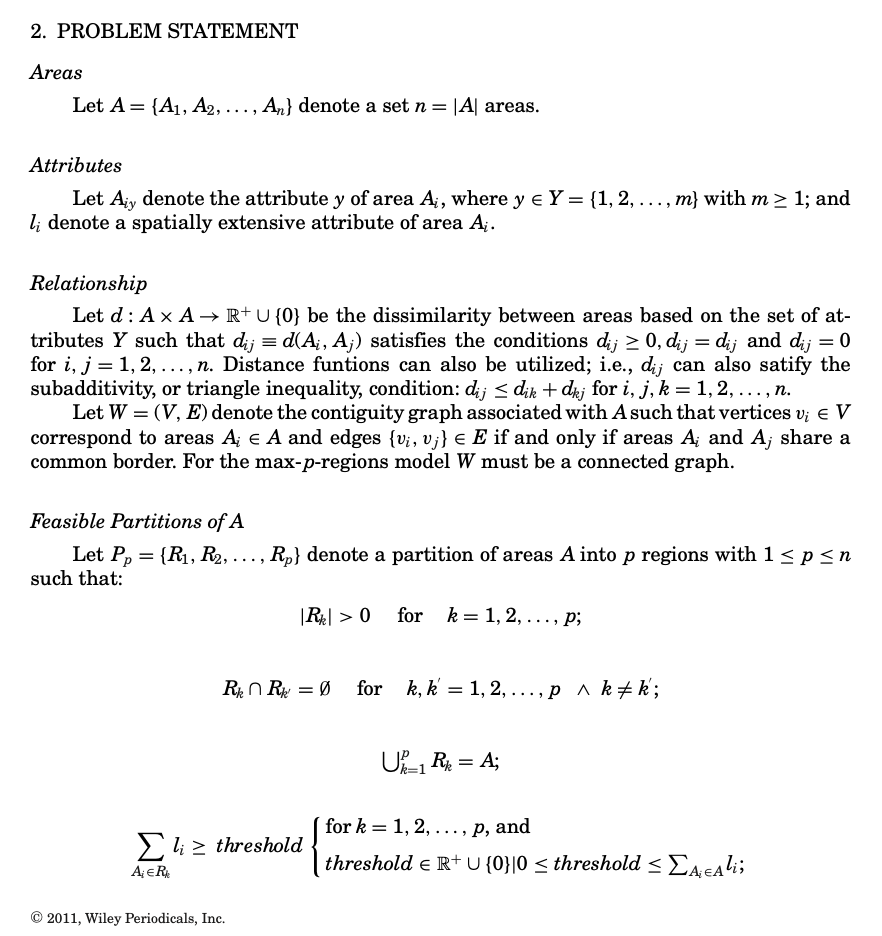
\includegraphics[width=0.70\textwidth]{problem_statement}
  \end{tabular}
\end{center}

\end{comment}

In a domain $\Omega\subset \mathbb{R}^2$  Quateroni\cite{quarteroni2009numerical} 
define incompressible Navier-Stokes Equations as follows 

\begin{equation}
  \begin{cases}
     \nabla \cdot \textbf{u} = 0 & \textbf{x} \in \Omega , t > 0\\
     
     \textbf{u}_t - \nabla \cdot[\nu (\nabla \textbf{u} + \nabla \textbf{u}^T)] + (\textbf{u}\cdot \nabla)
     \textbf{u}+ \nabla p = \textbf{f} & \textbf{x} \in \Omega , t > 0
  
  \end{cases}
  \label{1}
\end{equation}\\

When $\nu$ is constant, we obtain

$$\nabla \cdot[\nu (\nabla \textbf{u} + \nabla \textbf{u}^T)] = \nu (\Delta \textbf{u} + \nabla(\nabla \cdot \textbf{u})) = \nu \Delta \textbf{u}$$

and therefore the equations are written as

\begin{equation}
  \begin{cases}
     \nabla \cdot \textbf{u} = 0 & \textbf{x} \in \Omega , t > 0\\
     
     \textbf{u}_t - \nu \Delta \textbf{u} + (\textbf{u}\cdot \nabla)
     \textbf{u}+ \nabla p = \textbf{f} & \textbf{x} \in \Omega , t > 0
  
  \end{cases}
  \label{2}
\end{equation}\\

Being $\textbf{u}$ the fluid velocity field, $p$ the pressure divided by the density $\rho$, $\nu$
the kinematic viscosity define as $\frac{\mu}{\rho}$ with $\mu$ being the dynamic viscosity and $\textbf{f}$ 
a forcing term per unit mass.\\~\\
For the purpose of this work the domain $\Omega$ must also be bounded, and it is therefore necessary 
to assign initial and suitable boundary conditions for the problem to be well posed.

$$\begin{cases}
  \textbf{u}(\textbf{x},0) = \textbf{u}_0(\textbf{x}) & \forall \textbf{x} \in \Omega \\
  \textbf{u}(\textbf{x},t) = \varphi(\textbf{x},t) & \forall \textbf{x}\in \varGamma_D, t>0 \\
  \left(\nu\frac{\partial \textbf{u}}{\partial \textbf{n}}-p\textbf{n}\right)(\textbf{x},t) = \psi(\textbf{x},t) & \forall \textbf{x}\in \varGamma_N, t>0

\end{cases}$$

Where $\textbf{u}_0$ is a divergence free vector field,  $\varphi$ and $\psi$ are given vector
functions, $\varGamma_D$ and $\varGamma_N$ provide a partition of the boundary $\partial \Omega$ and 
\textbf{n}, as usual, represents the outward unit normal vector to $\partial \Omega$.

\section{Objectives}

\subsection{General objective}

\begin{comment}
  (\textcolor{red}{sólo uno})
  El objetivo general enmarca todo el trabajo. Está estrechamente relacionado con el
título y con la pregunta de investigación y describe de intensión de la
invesstigación.

La estructura de un objetivo general es la siguiente: verbo en infinitivo (uno
solo) + qué (objeto de estudio) + cómo + para qué.
\end{comment}

Compare the performance of Neural Network asisted Reduced Basis Models (NN-RBMs) and Physical Informed Neural Networks (PINNs)
agains the Finite Element Method on a real-time context, by performing multiple simulations 
of the blood flow through the carotid arthery.

\subsection{Specific objectives}

\begin{comment} 
  (\textcolor{red}{3 o 4 objetivos})
  Son un conjunto de objetivos más pequeños que permitirán alcanzar el general.
  La estructura de un objetivo general es la siguiente: Verbo en infinitivo (uno
  solo) + qué (objeto de estudio) + cómo.

  Importante: los objetivos específicos no se pueden confundir con una lista de
  tareas. El objetivo debe comenzar con un fin/logro no con el medio/actividad
  (las actividades van en la metodología); por ejemplo, un objetivo específico
  del tipo ``Realizar una revisión bibliográfica para...'' debería transformarse
  en algo como ``Encontrar información científica por medio de una revisión
  sistemática de la literatura''.

\end{comment}

\begin{itemize}
  \item Identify the principal differences on the implementation of NN-RBMs and PINN like models and FEM in a fluid mechanic context.
  \item Assess the ability of NN-RBMs and PINNs to adapt to changing boundary conditions or parameters, compared to the FEM approach.
  \item  Study the generalization capabilities of NN-RBMs and PINNs when trained on a specific set of data and tested on different scenarios, compared to FEM.
  \item Analyze the dependency of NN-RBMs to the Snapshots used for the training on the model
\end{itemize}

\section{Justification}

\begin{comment}

En esta sección se argumenta el por qué es importante resolver el problema o
contestar la pregunta de investigación. Las argumentaciones pueden ser de tipo
teórico o práctico y soportadas en literatura.

\begin{itemize}
\item Destaca los beneficios derivados del aporte (¿para qué servirá esta investigación?, ¿qué aporta de nuevo esta investigación?, ¿cuáles son los beneficios?, ¿quiénes serán los beneficiados y de qué modo?, ¿qué se prevé cambiar con la investigación?, ¿cuál es la utilidad?, ¿resolverá algún problema práctico?, ¿se cubrirá algún gap de conocimiento?, ¿los resultados se podrán generalizar?, ¿sirve para apoyar alguna teoría?, ¿permite un mejor estudio de una población o fenómeno?, ¿se pueden establecer plazos para los beneficios?). OJO: las preguntas no se incluyen en el cuerpo del texto, son sólo una guía para encontrar los argumentos.
\item Las respuestas a estas preguntas deben considerar tres aspectos: teórico, práctico y metodológico.
\end{itemize}

\end{comment}

\textcolor{red}{ Finally, this project aims to contribute to a deeper understanding of the advantages and limitations of neural NN-RBMs, PINNs and FEM in the context of real-time simulations of the Navier-Stokes equations. Guiding researchers and practitioners in selecting the most appropriate method for specific applications based on accuracy and computational efficiency considerations.}\\

\section{Scope}

\begin{comment}
  \textcolor{red}{2 o 3 párrafos})

  Describe las principales barreras o limitaciones de la investigación,
  así como las principales herramientas y otros recursos que esperaba utilizar
  durante la ejecución del proyecto. También describe los principales
  resultados esperados de la investigación
\end{comment}



Now then, it is clear that for this kind of project one of the biggest obstacles that it is possible
to encounter when researching and implementing the model is the impossibility of carrying out
analytical validation of the solution obtained by the method, since as it is known, the Navier-Stokes
equations, due to their high complexity, do not have an analytical solution against which to compare
the numerical solution. However, since multiple models are implemented, and having the FEM as a commontly
accepted method for the solution of Parameterized PDEs, it's solution will be used as an accepted solution 
for validating the implemented models. 

\section{State of the art}

\begin{comment}
(\textcolor{red}{5 a 6 párrafos})
Describe las principales referencias relacionadas con el problema. Este estado
del arte puede referirse al problema o aplicación específica, o bien a los
métodos aplicados para solucionarlo. No debes olvidar incluir los trabajos más
importantes y los más recientes.

\end{comment}


\section{Proposed methodology}

\begin{comment}

 (\textcolor{red}{5 o 6 párrafos})
Describe en este apartado los métodos, técnicas, algoritmos, etc. que se
utilizarán durante la ejecución del proyecto.

Incluye aspectos como:

\begin{itemize}
\item ¿Qué métodos se suelen usar para responder la pregunta de investigación?
\item ¿Por qué seleccionaste el método que usarás?
\item Describe el método: Supuestos básicos, ventajas y desventajas del método.
\end{itemize}
\end{comment}

As a means to achieve the objectives set for this project, a 4-stage methodology is proposed in which
various mathematical methods will be worked. In the first stage, the interpretation of angiograms
obtained on the web will be performed and then a two-dimensional geometry of the carotid artery will
be recreated to be used as the spatial domain of the simulations to be performed. In the second stage, 
a computational implementation of the finite element method for obtaining an initial solution for the 
implementation and validation of the other models. The third stage involves the implementation of NN-RBMs and 
PINNs using the results obtained before as a basis for this models and the simulation fo multiple study 
cases. And finally, in the fourth stage, a comparison of the results obtained for each implmented model, as well as their simulation-time and memory usage is performed, to analyze the performance of each model.\\





\section{Schedule, commitments and deliverables}

\begin{comment}

\begin{itemize}
\item Cronograma de las actividades a realizar durante la PI.
\item Compromisos entre el tutor y el estudiante (e.g., periodicidad de
    reuniones, entrega de datos, etc.).
\item Lista clara de entregables que se esperan de la práctica.
\end{itemize}

Adapta es siguiente cronograma a tu PI.

\end{comment}


\begin{table}[h!]
	\begin{center}
     \caption{Schedule}
	\label{tb_sch}
       
    \scalebox{0.78}{
    \normalsize{
		\begin{tabular}{|p{7cm}|r|r|r|r|r|r|r|r|r|r|r|r|r|r|r|r|r|r|}
			\hline
			\multirow{2}{*}{\emph{Activity}} & \multicolumn{18}{c|}{\emph{Weeks}} \\
			\cline{2-19}
            & \emph{\footnotesize 1} & \emph{\footnotesize 2} & \emph{\footnotesize 3} & \emph{\footnotesize 4} & \emph{\footnotesize 5} & \emph{\footnotesize 6} & \emph{\footnotesize 7} & \emph{\footnotesize 8} & \emph{\footnotesize 9} & \emph{\footnotesize 10} & \emph{\footnotesize 11} & \emph{\footnotesize 12} & \emph{\footnotesize 13} & \emph{\footnotesize 14} & \emph{\footnotesize 15} & \emph{\footnotesize 16} & \emph{\footnotesize 17} & \emph{\footnotesize 18} \\
			\hline
			Literature Review & \cellcolor{black}{1}  & \cellcolor{black}{1} & \cellcolor{black}{1} & \cellcolor{black}{1} & \cellcolor{black}{1} &  &  &  &  &  &  &  &  &  &  &  &  &  \\
			\hline
			Research proposal writting & & & &  & \cellcolor{black}{1} & \cellcolor{black}{1} & & & & & & & & & & & & \\
			\hline
			Activity 3 & & & & & & & & & \cellcolor{black}{1} &  \cellcolor{black}{1}& \cellcolor{black}{1} & \cellcolor{black}{1} & & & & & & \\
			\hline
			Results Analysis and comparison & & & & & & & & & & & & & \cellcolor{black}{1} & \cellcolor{black}{1} & \cellcolor{black}{1} & & & \\
			\hline
			Final Report writting & & & & & & & & & & & & & & & & \cellcolor{black}{1} & \cellcolor{black}{1} & \cellcolor{black}{1} \\
			\hline
		\end{tabular}
        }
        }
	\end{center}
\end{table}

\section{Intellectual property}

According to the internal regulation on intellectual property within
Universidad EAFIT, the results of this research practice are product of
\emph{Alejandro Salazar Arango} and \emph{Cristhian David Zambrano Mora}.\\

In case further products, beside academic articles, that could be generated from this work, the intellectual property distribution related to them will be directed under the current regulation of this matter determined by \cite{reglamento2017}.

\bibliographystyle{vancouver}
\bibliography{references.bib}

\end{document}
